%#!platex 000main.tex
\chapter{システム構成}
  \label{chap:system}
  \section{ハードウェア}
  	\label{chap:hardware}
 	ロボットの機体はAdeeptのADA031というモデル名の簡易用のキッドを購入した. Arduinoで動作するが,画像処理が難しかったため,基盤をRaspberry Piに代えた. またロボットアームに接続しているサーボモータを動かすのにブレッドボードやジャンパー線、抵抗を用意した.
  \section{機構}
  	\label{chap:mechanism}
	本研究で用いるロボットは3軸のマニピュレータロボットである. servo1の回転軸を原点とし,各サーボモータの回転角度を$\theta_1,\theta_2,\theta_3$,各リンクの長さを$l_1,l_2,l_3,l_4$とする. 図3.1はリンク座標系の定義と,実機の様子を示したものである.
		 \begin{center}
        \begin{figure}[h]
            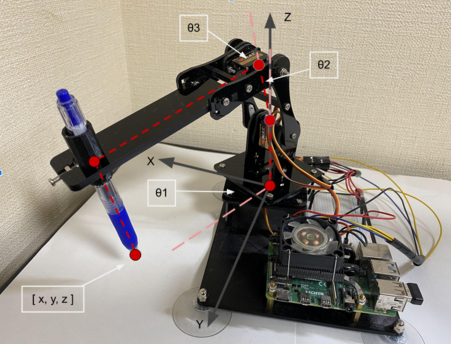
\includegraphics[width=1.0\textwidth]{./img/004.png}
            \caption{各関節角と手先位置の関係}
            \label{test}
        \end{figure}
    \end{center}

  \section{手先の位置と回転角の関係}
  	\label{chap:kinetic}
	リンク座標系に定義した各パラメータと,順運動学と逆運動学を用いて手先の位置から回転角を求める. 今回はDH(Denavit-Hartenberg)記法を用いて,各リンクの関係を示す.
	このリンク座標系をもとに,座標系1から3への座標変換行列を求めると以下のようになる.
	\begin{equation}
		\boldsymbol{ ^{0}T_{3}=^{0}T_{1} ^{1}T_{2} ^{2}T_{3} }
		\begin{array}{cc}
			=
			\left(
				\begin{array}{cccc}
					C_1C_{23} & -C_1S_{23} & 0 & l_2C_1S_2 \\
					S_1C_{23} & -S_1S_{23} & 0 & l_2S_1S_2 \\
					-S{23} & -C_{23} & -1 & l_2C_2 + l_1 \\
					0 & 0 & 0 & 1
				\end{array}
			\right)
		\end{array}
	\end{equation}
	ただし,
	\begin{equation*}
		\begin{split}
			C_{23} = cos\theta_2cos\theta_3-sin\theta_2sin\theta_3\\
			S_{23} = sin\theta_2cos\theta_3+cos\theta_2sin\theta_3
		\end{split}
	\end{equation*}
    また,手先ベクトルが以下のように求まる.
	\begin{equation}
	\begin{array}{cccc}
		&\left(
			\begin{array}{cccc}
				1 & 0 & 0 & l_4\\
				0 & 1 & 0 & 0\\
				0 & 0 & 1 & 0\\
				0 & 0 & 0 & 1
			\end{array}
		\right)
		\left(
			\begin{array}{cccc}
				1 & 0 & 0 & 0\\
				0 & 1 & 0 & -l_3\\
				0 & 0 & 1 & 0\\
				0 & 0 & 0 & 1
			\end{array}
			\right)
		&=
		\left(
		\begin{array}{cccc}
			1 & 0 & 0 & l_4\\
			0 & 1 & 0 & -l_3\\
			0 & 0 & 1 & 0\\
			0 & 0 & 0 & 1
		\end{array}
		\right)
	\end{array}
	\end{equation}
	式(3.1)と(3.2)より手先までの座標変換行列$\boldsymbol{ ^{0}P_{r} }$が以下のように求まる.
	\begin{equation*}
		\boldsymbol{ ^{0}P_{r} } =
		\boldsymbol{^{0}T_{3}}
		\left(
		\begin{array}{cccc}
			1 & 0 & 0 & l_4\\
			0 & 1 & 0 & -l_3\\
			0 & 0 & 1 & 0\\
			0 & 0 & 0 & 1
		\end{array}
		\right)=
		\begin{array}{cc}
			\left(
				\begin{array}{cc}
					\boldsymbol{R} & \boldsymbol{t} \\
					\boldsymbol{0} & 1
				\end{array}
			\right)
		\end{array}
	\end{equation*}
	ただし,回転行列$\boldsymbol{R}$と並進ベクトル$\boldsymbol{t}$は以下の結果になる.
	\begin{equation*}
	\begin{split}
		&\boldsymbol{R} =
		\begin{array}{cc}
			\left(
				\begin{array}{ccc}
					C_1C_{23} & -C_1S_{23} & 0 \\
					S_1C_{23} & -S_1S_{23} & 0 \\
					-S{23} & -C_{23} & -1
				\end{array}
			\right)
		\end{array} \\
		&\boldsymbol{t} =
		\begin{array}{cc}
			\left(
				\begin{array}{c}
					l_4C_1C_{23}+l_3C_1S_{23}+l_2C_1S_2 \\
					l_4S_1C_{23}+l_3S_1S_{23}+l_2S_1S_2 \\
				-l_4S_{23}+l_3C_{23}+l_2C_2+l_1
				\end{array}
			\right)
		\end{array}\\
		&\boldsymbol{0} =
		\begin{array}{cc}
			\left(
				\begin{array}{ccc}
					0 & 0 & 0
				\end{array}
			\right)
		\end{array}
	\end{split}
	\end{equation*}

	座標変換行列の並進ベクトル$\boldsymbol{t}$が順運動学解なので,手先の位置x,y,zが以下のように求まる.
	\begin{equation}
			\begin{array}{c}
			\begin{split}
				x &=& C_1(l_4C_{23} + l_3S_{23} + l_2S_2) \\
				y &=& S_1(l_4C_{23} + l_3S_{23} + l_2S_2) \\
				z - l_1 &=& -l_4S_{23} + l_3C_{23} + l_2C_2
			\end{split}
		\end{array}
	\end{equation}
	式(3.3)より逆運動学解$\theta_1,\theta_2,\theta_3$は以下のように求まる.
	\begin{equation}
			\begin{array}{c}
			\begin{split}
				\theta_1  &  =\frac{1}{2}  cos^{-1}\biggl( \frac{x^2-y^2}{x^2+y^2} \biggr) \\
				\theta_2 & = cos^{-1}\biggl( \frac{x^2+y^2+(z-l1)^2 + l_2^2-l_3^2-l_4^2}{2l_2\sqrt{x^2+y^2+(z-l_1)^2}} \biggr) + tan^{-1}\biggl( \frac{\sqrt{x^2+y^2}}{z-l1}\biggr) \\
				\theta_3 & =cos^{-1}\biggl( \frac{x^2+y^2+(z-l1)^2 - l_4^2-l_3^2-l_2^2}{2l_2\sqrt{l_3^2+l_4^2}}\biggr) + tan^{-1}\biggl( \frac{-l_4}{l_3}\biggr)
			\end{split}
			\end{array}
	\end{equation}
	\section{画像処理}
	線画を描くためにエッジの抽出を行った. エッジの抽出には様々なアルゴリズムが提案されているが,今回は代表的なケニーのエッジ検出アルゴリズムとガウシアンラプラシアンフィルターを比較し,ノイズが少なく綺麗にエッジ抽出を行えている方を用いることにする. 
	文献\cite{4}も比較したかったのだが,実装できなかったので,今回はOpenCVのCannyのエッジ検出器とガウシアンラプラシアンに細線化を行った2つを比較した. 以下のそれぞれのエッジ抽出の結果を示す. 
	 \begin{center}
        \begin{figure}[h]
            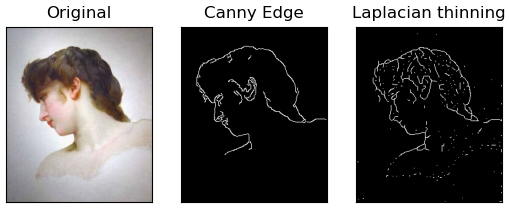
\includegraphics[width=1.0\textwidth]{./img/001.png}
            \caption{エッジ抽出}
            \label{manipulator}
        \end{figure}
    \end{center}
	図の3.1からラプラシアンフィルタより,Cannyの方がノイズが少なく綺麗にエッジ抽出できていることが分かる. そのため,Cannyでエッジ抽出を行った結果を線画とする. この出力画像をもとに線の経路を求めていく.
